\section{Background}
\label{sec:background}

\subsection{Preliminaries and problem statement}
\label{sec:intro-problem}

We consider labeled graphs $G=(V_G,E_G,L,\ell_G)$, where $V_G$ and $E_G$ are the sets of
nodes and edges, $L$ is a set of labels and $\ell_G: V \rightarrow L$ is a labeling
on the nodes.  A graph $H=(V_H, E_H, L, \ell_H)$ is a \emph{non-induced
subgraph} of $G$ if we have $V_H\subseteq V_G$ and $E_H\subseteq E_G$.  We
say that a template graph $T = (V_T, E_T, L, \ell_T)$ is isomorphic to a non-induced
subgraph $H = (V_H,E_H, L, \ell_H)$ of $G$ if there exists a bijection
$f: V_T \rightarrow V_H$ such that: (i) for each $(u, v) \in E_T$, we have
$(f(u), f(v))\in E_H$, and (ii) for each $v \in V_T$, we have
$\ell_T(v) = \ell_H(f(v))$. In this paper, we assume $T$ is a tree. We will consider trees to be rooted,
and use $\rho=\rho(T)\in V_T$ to denote the ``root'' of $T$, which is arbitrarily chosen.
If $T$ is isomorphic to a non-induced subgraph $H$ with the mapping $f(\cdot)$,
we also say that $H$ is a non-induced embedding of $T$ with the root $\rho(T)$
mapped to node $f(\rho(T))$.
Figure~\ref{fig:isomorphism} shows an example of a non-induced embedding of template
$T$ in a graph $G$.
Let $emb(T, G)$ denote the number of all embeddings of template $T$ in graph $G$.
Here, we focus on approximating $emb(T, G)$.

\begin{figure}[htbp]
\centerline{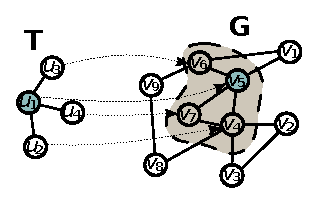
\includegraphics[width=0.35\textwidth]{plots/isomorphism.eps}}
\caption{Here the shaded subgraph is a non-induced embedding of T. The mapping
of the template to the subgraph is denoted with the arrow.}
\label{fig:isomorphism}
\end{figure}

%\subsection{$(\varepsilon,\delta)$-approximation}

\smallskip
\noindent
\textbf{An $(\varepsilon,\delta)$-approximation to $emb(T,G)$.}
We say that a randomized algorithm $\mathcal{A}$ produces an
\emph{$(\varepsilon,\delta)$-approximation} to $emb(T,G)$, if the estimate $Z$
produced by $\mathcal{A}$ satisfies: $\Pr[|Z-emb(T,G)|>\varepsilon \cdot
emb(T,G)]\leq 2\delta$; in other words, $\mathcal{A}$ is required to produce an
estimate that is close to $emb(T, G)$, with high probability.

\smallskip
\noindent
\textbf{Problems studied.}
We consider the following two problems:
\begin{enumerate}
\item
\emph{Subgraph counting}: 
Given a template $T$ and graph $G$, compute an $(\varepsilon,\delta)$-approximation to $emb(T,G)$.
When the labels can be disregarded, we refer to this as the \emph{Unlabeled Subgraph Counting}
problem. Otherwise, it is referred to as the \emph{Labeled Subgraph Counting} problem.
\item
\emph{Graphlet Frequency Distribution (GFD)}~\cite{przulj2007biological}:
a graphlet is another name for a subgraph. We say a node touches a graphlet $T$,
if it is contained in an embedding of $T$ in the graph $G$. The
graphlet degree of a node $v$ is the number of graphlets it touches.
Given a size parameter $k$, the GFD in a graph $G$ is the frequency distribution
of the graphlet degrees of all nodes with respect to all graphlets of size up to $k$. 
The specific problem is to obtain an approximation to the GFD.
In this paper, we will focus on ``treelets'', which only considers all trees of size up to $k$.
\end{enumerate}

\subsection{MapReduce, Hadoop and Harp}
\label{sec:intro-map-reduce}

MapReduce and its extensions have become a dominant computation model
in big data analysis.  It involves two stages for data processing: (a)
divide the input into distinct \emph{map} tasks and distribute to
multiple computing entities, and (b) merging the results of individual
computing entities in the \textit{reduce} tasks to produce the final
output~\cite{dean2008mapreduce}.

The MapReduce model processes data in the form of key-value pairs
$\langle k, v \rangle$. An application first takes pairs of the form
$\langle k_1, v_1 \rangle$ as input to the map function, in which one or
more $\langle k_2, v_2 \rangle$ pairs are produced for each input
pair.  Then the MapReduce re-organizes all $\langle k_2, v_2 \rangle$
pairs and aggregates all items $v_2$ that are associated with the same
key $k_2$, which are then processed by a reduce function.

Hadoop~\cite{white2010hadoop} is an open-sourced implementation of
MapReduce.  By defining application specific map and reduce functions,
the user can employ Hadoop to manage and allocate appropriate
resources to perform the tasks, without knowing the complexity of load
balancing, communication and tasks scheduling. Due to the reliability
and scalability in handling vast amount of computation in parallel,
Hadoop is becoming a \emph{de facto} solution for large parallel
computing tasks.

Hadoop falls short in two aspects though: ({\it i}) the high I/O cost
involved within mapper, shuffling and reducer since the data is always
read and write from the disk in every stage of a Hadoop job and ({\it ii})
global synchronization in mapper and reducer, i.e. reducers can start
only when all mappers have completed their tasks and vice versa,
reduce the efficient usage of the computing resources. To conquer the
problems that Hadoop is facing, we further extends our work to use the
Harp platform~\cite{qiu2014towards}.

Harp introduces full collective communication (broadcast, reduce,
allgather, allreduce, rotation, regroup or push \& pull), adding a
separate communication abstraction. The advantage of using in-memory
collective communication replacing the shuffling phase is that
fine-grained data alignment and data transfer of many synchronization
patterns can be optimized.

Harp categorizes four types of computation models (Locking, Rotation,
Allreduce, Asynchronous) that are based on the synchronization
patterns and the effectiveness of the model parameter update. They
provide the basis for a systematic approach to parallelizing iterative
algorithms. Since the ``Rotation'' model partitions the global model
parameters among distributed workers, it effectively reduces the
memory footprint but requires model synchronization using collective
communication. Figure~\ref{fig:harp} shows the four categories of the
computing model.

\begin{figure}[htbp]
\centerline{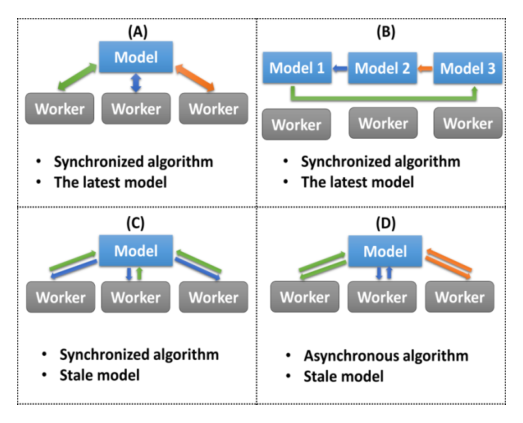
\includegraphics[width=0.35\textwidth]{plots/harp.eps}}

\caption{Harp has 4 computation models: (A) Locking,(B)Rotation, (C) AllReduce, (D) Asynchronous}

\label{fig:harp}
\end{figure}

The Harp framework has been used by 350 students at Indiana University
for their course projects. Now it has been released as open source
project that is available at public github domain
\cite{Web:harp}. Harp provides a collection of iterative machine
learning and data analysis algorithms (e.g. Kmeans, Multi-class
Logistic Regression, Random Forests, Support Vector Machine, Neural
Networks, Latent Dirichlet Allocation, Matrix Factorization,
Multi-Dimensional Scaling) that have been tested and benchmarked on
OpenStack Cloud and HPC platforms including Haswell and Knights
Landing architectures. It has also been used for Subgraph mining,
Force-Directed Graph Drawing, and Image classification applications.

